\documentclass{article}

\usepackage[margin=1in]{geometry}
\usepackage{amsmath,amssymb,amsthm}
\usepackage{graphicx}
\usepackage[round]{natbib}
\usepackage{booktabs}
\usepackage{hyperref}
\usepackage{xcolor}
\usepackage{caption}
\usepackage{subcaption}
\usepackage{enumitem}

\title{Cost-Constrained Edge Removal for Epidemic Containment on Social Networks:\\
A Comparison of Heuristic and GNN-Learned Policies on Facebook100}

\author{Karlo Vran\v{c}i\'{c}, Alec [Last], Jackson Webster, Ryan [Last]\\
STAT 175 (Prof. Morgane Austern), Harvard University}

\date{\today}

\begin{document}
\maketitle

\begin{abstract}
We study cost-constrained epidemic containment on real social networks
(Facebook100) under a stochastic Susceptible-Infected-Susceptible (SIS)
model. Edge removal is the intervention modality and the cost of
removing an edge is derived from the similarity of the two endpoints'
feature vectors via a sigmoid-dot-product proxy. We compare four
policies: random, edge betweenness over cost, a Louvain-community
``distance threshold'' (the realistic implementable form), and a
graph neural network (GNN) policy that learns node embeddings whose
similarity is the per-edge cost.  We sweep cost budgets to recover
Pareto frontiers of cost vs.\ steady-state prevalence on five
Facebook100 campuses, run robustness panels (SIR alternative,
imperfect compliance, adversarial seeding) and three ablations
(GNN architecture, cost function, synthetic graph topology), and
fit a cross-campus regression of policy AUC against descriptive
graph statistics. We discuss when the GNN-learned cost beats the
hand-designed cost, when classical betweenness suffices, and how
much we lose by constraining ourselves to enforceable rules.
\end{abstract}

\section{Introduction}
\label{sec:intro}

\paragraph{Scientific question.}
\emph{Given a social contact graph in which vertices carry feature
information and edges carry costs derived from endpoint feature
similarity, what is the minimum-cost set of edges whose removal keeps
the steady-state SIS prevalence below a fixed threshold?}

\paragraph{Motivation for the cost-aware reframe.}
The classical literature on epidemic containment via network
modification studies the \emph{cardinality} version of this problem:
remove the minimum number of edges, or equivalently the maximum-impact
$k$ edges, such that the residual graph's spectral radius drops below
the epidemic threshold $\tau_c = 1/\lambda_1(A)$
\citep{wang2003threshold,tong2012netmelt,saha2015greedywalk}. The
cardinality formulation treats every edge as identical. In real social
graphs this is unrealistic: cutting the friendship between two
roommates is socially much costlier than cutting an acquaintance tie
across a campus. A containment policy that ignores this asymmetry is
either practically impossible to deploy (it severs critical ties) or
underutilizes cheap interventions (it misses harmless cuts that would
still bend the curve). The cost-aware reframe takes node features as
input, derives a per-edge cost from those features, and minimizes the
total cost of the edges removed subject to a containment constraint.

\paragraph{Contributions.}
\begin{enumerate}[leftmargin=2em]
    \item An end-to-end empirical comparison of four edge-removal
    policies (random, edge betweenness over cost, a Louvain-induced
    community-distance threshold, and a GNN-learned cost policy) on
    five Facebook100 campuses chosen for diversity in clustering
    coefficient.
    \item A graph neural network policy whose per-edge cost
    $c_e^{\textsc{gnn}} = \sigma(\langle z_u, z_v\rangle)$ is
    \emph{learned} from a self-supervised link-prediction objective on
    the friendship graph itself. The GNN converts attribute-driven
    homophily into a continuous cost surface, and the learned cost is
    combined with NetMelt-style spectral edge importance into a
    single bang-for-buck score.
    \item An implementability analysis: we report the gap between the
    ideal policy (GNN over cost) and a realistic, enforceable policy
    (community-distance threshold), under both perfect and imperfect
    compliance.
    \item Three robustness panels (SIR alternative, $80\%$
    compliance, adversarial top-eigenvector seeding) and three
    ablations (GNN architecture, cost function, synthetic graph
    topology) that characterize \emph{when} each policy wins.
\end{enumerate}

\section{Background}
\label{sec:background}

\subsection{Graph and SIS dynamics}

Let $G = (V, E)$ be an undirected graph with $n = |V|$ vertices and
$m = |E|$ edges, and let $A \in \{0, 1\}^{n \times n}$ be its
adjacency matrix. Each vertex $v \in V$ carries a feature vector
$x_v \in \mathbb{R}^d$ (in our case the L2-normalized one-hot
encoding of seven Facebook100 attributes). At each discrete time
step, every infected node infects each susceptible neighbor
independently with probability $\beta$ per edge, and recovers (back
to susceptible) with probability $\gamma$. Equivalently, a
susceptible vertex with $k$ infected neighbors becomes infected
with probability $1 - (1 - \beta)^k$.

The SIS model has a phase transition governed by the leading
eigenvalue of $A$. \citet{wang2003threshold} showed that the
quenched mean-field epidemic threshold is
\[
    \tau_c = \frac{1}{\lambda_1(A)}.
\]
For $\beta/\gamma < \tau_c$ the epidemic dies out almost surely; for
$\beta/\gamma > \tau_c$ a positive-prevalence endemic state
persists. Controlling the leading eigenvalue therefore controls
containment: removing edges that contribute most to $\lambda_1(A)$
is the classical recipe for raising $\tau_c$ above $\beta/\gamma$.

We work in the stochastic (per-vertex Bernoulli) version of SIS and
define our primary outcome as the time-averaged
\emph{steady-state prevalence}: the fraction of infected vertices
averaged over a post-burn-in window of the simulation.

\subsection{Cost-aware edge removal as a constrained optimization
problem}

Let $c : E \to \mathbb{R}_{\geq 0}$ be a per-edge cost function. For
any subset $S \subseteq E$ define the total cost
$C(S) = \sum_{e \in S} c_e$ and write $G \setminus S$ for the
residual graph after removing the edges in $S$. Let
$\textrm{Outcome}(G_S)$ be the steady-state prevalence of an SIS
process on $G \setminus S$ at fixed $(\beta, \gamma)$. The
constrained optimization problem we study is
\[
    \min_{S \subseteq E} \quad C(S)
    \qquad \textrm{s.t.} \quad
    \textrm{Outcome}(G \setminus S) \le \tau,
\]
or equivalently in budgeted form
\[
    \min_{S \subseteq E} \quad \textrm{Outcome}(G \setminus S)
    \qquad \textrm{s.t.} \quad
    C(S) \le B,
\]
where $\tau$ is a containment target and $B$ a cost budget. We sweep
$B$ over a logarithmic grid and report the implied Pareto frontier.
This is a generalization of the cardinality formulation of
\citet{tong2012netmelt} and \citet{saha2015greedywalk}; the
non-uniform costs are what make the problem genuinely cost-aware.

\subsection{The cost proxy}
\label{sec:cost-proxy}

We follow our advisor's suggestion and the social network analysis
literature on homophily \citep{newman2002assortative,
rizi2025homophily} in defining the per-edge cost as a smooth
function of endpoint feature similarity:
\[
    c_e \;=\; \sigma\!\left(\langle x_u, x_v\rangle\right),
\]
with $x_u, x_v$ the L2-normalized one-hot feature vectors of edge
$e = (u, v)$ and $\sigma(\cdot)$ the logistic sigmoid. Edges between
nodes with strongly aligned attribute profiles (same dorm, same
year, same major) inherit a high cost; edges between dissimilar
nodes are cheap. The L2 normalization ensures
$\langle x_u, x_v \rangle \in [0, 1]$, so $c_e \in
[\tfrac{1}{2}, \sigma(1)] \approx [0.5, 0.73]$. The cost function's
limited dynamic range is a known limitation that we address in the
ablation in Section~\ref{sec:results}.

\section{Related work}
\label{sec:related}
% [DRAFT] Anchor papers from useful-readings-A.md sec 3 (Tong/NetMelt
% 2012, Saha/GreedyWalk 2015, Yi 2022 supermodularity) and frontier from
% useful-readings-B.md sec 1-2 (Li-Eliassi-Rad SDM 2024, MIND 2025,
% Liu KDD 2024 GNN+epidemic survey, Block et al. 2020 social
% distancing strategies, Rizi/Stegehuis/Kivela Nature Comm 2025
% homophily-and-percolation). For each anchor cite arxiv id from
% the readings, fetched via the arxiv MCP per Karlo's note in the
% approved plan.

\section{Methods}
\label{sec:methods}

\subsection{Edge cost}

We L2-normalize the concatenated one-hot encoding of seven
Facebook100 attributes per node (student/faculty status, gender,
major, second major, dorm, year, high school) and treat missing
values (coded $0$ in the dataset) as their own category to avoid
biasing the encoding through imputation
\citep{traud2012facebook100}. The primary per-edge cost is then
$c_e = \sigma(\langle x_u, x_v\rangle)$ as defined in
Section~\ref{sec:cost-proxy}. The robustness panel additionally
considers (i) a uniform cost (recovering the cardinality
formulation), (ii) cosine similarity rescaled to $[0, 1]$, (iii) a
clipped raw dot product, and (iv) an oracle log-normal cost
independent of features.

\subsection{The four policies}

Every policy implements a uniform interface
$P : (G_S, c, B) \to S \subseteq E$ that returns the indices of edges
to remove given a residual graph, a cost vector, and a cost budget.

\paragraph{Random edge removal.} The trivial baseline. Edges are
drawn uniformly without replacement until the cumulative cost
reaches~$B$.

\paragraph{Edge betweenness over cost.} For each edge $e$ we
compute its (approximate) betweenness centrality $b_e$ via Brandes'
algorithm with $k = 300$ pivot sources \citep{tong2012netmelt}. We
score each edge by $b_e / c_e$ and greedy-fill in descending score
order until the budget is exhausted. Sampled betweenness is a
documented approximation; the variance under different pivot draws
is captured by the pinned random seed.

\paragraph{Distance threshold (community-bubble cut).} Run Louvain
\citep{blondel2008louvain} on the residual graph to obtain a
partition. Build the community meta-graph whose nodes are
communities and whose edges connect any pair of communities sharing
at least one inter-community edge. For each original edge $(u, v)$
with community labels $c_u, c_v$, define its meta-graph distance
$d_{c_u, c_v}$ as the BFS hop count between the two communities
(with $d = 0$ if $c_u = c_v$). Score each edge by
$d_{c_u, c_v} / c_e$ and greedy-fill until budget. This is the
realistic, enforceable form: a public-health intervention can in
principle communicate "stay within your $k$-hop community bubble"
to the population.

\paragraph{GNN-learned cost (the novel contribution).} A 2-layer
GraphSAGE encoder \citep{hamilton2017graphsage} produces 16-dim
node embeddings $z_v$. Cost from learned space:
$c_e^{\textsc{gnn}} = \sigma(\langle z_u, z_v\rangle)$. Structural
impact is the NetMelt eigenscore $2 u_i u_j$, the first-order
perturbation of $\lambda_1(A)$ when edge $(i, j)$ is removed, where
$u$ is the leading eigenvector of $A$
\citep{tong2012netmelt}. Edges are scored by
$2 u_i u_j / c_e^{\textsc{gnn}}$ and greedy-filled until budget.

The encoder is trained end-to-end via self-supervised link
prediction: for each true edge we sample a random non-edge as a
negative; the loss is binary cross-entropy on the logit
$\langle z_u, z_v \rangle$. We project the high-dimensional one-hot
features through a 64-component TruncatedSVD before the GraphSAGE
layers so that per-epoch cost does not scale with the raw feature
dimension. Training takes under 40 seconds total across the five
campuses.

The GNN policy's novelty is that the cost function itself is
\emph{learned} from data rather than hand-designed; the training
signal aligns the cost surface with the graph's homophily structure
without ever consulting the SIS simulator.

\section{Experimental setup}
\label{sec:setup}

\paragraph{Datasets.} We use five Facebook100 campuses chosen for
diversity in global clustering coefficient: Caltech36 (762 nodes),
Bowdoin47 (2{,}250), Harvard1 (15{,}086), Penn94 (41{,}536), and
Tennessee95 (16{,}977). Each network is restricted to its giant
connected component before any analysis.

\paragraph{Epidemic regime.} We fix $\gamma = 0.10$ and parameterize
$\beta$ via the basic reproduction number
$R_0 = \beta \lambda_1(A) / \gamma$ so that the regime is comparable
across campuses of very different size. We sweep
$R_0 \in \{0.8, 1.5, 3.0, 6.0\}$, which brackets the spectral
threshold ($R_0 = 1$) and reaches into the strongly endemic regime.

\paragraph{Simulation.} Each Pareto cell runs $N = 50$ stochastic
SIS realizations of $200$ time steps each, with $10$ uniformly
random initial-infected vertices per realization, and we discard
the first $100$ steps as burn-in before time-averaging steady-state
prevalence. Random seeds are pinned to $42$ throughout
(\texttt{numpy}, \texttt{torch}, \texttt{python-louvain}, and the
betweenness pivot sampler all derive from the same master seed).

\paragraph{Budget grid.} For each cell we sweep the cost budget at
$\{0\%, 0.5\%, 1\%, 2\%, 5\%, 10\%, 20\%, 40\%\}$ of the total cost,
yielding a Pareto frontier of cost vs.\ steady-state prevalence per
$(campus, R_0, policy)$.

\paragraph{Reproducibility.} Every figure in this paper is
regenerated by \texttt{python scripts/08\_make\_figures.py} from
parquet result tables in \texttt{results/}; every parquet is
produced by the corresponding numbered script. The full
end-to-end pipeline from raw \texttt{.mat} download to final
figures runs from a single command sequence documented in
\texttt{README.md}.

\section{Results}
\label{sec:results}

\subsection{Main Pareto frontiers}

We sweep $5$ campuses $\times$ $4$ policies $\times$ $4$ values of
$R_0$ $\times$ $8$ budget fractions, with $N = 50$ stochastic SIS
realizations per cell ($6{,}400$ Pareto cells; $640$ rows after
collapsing across realizations). All headline numbers below are
mean steady-state prevalences with $95\%$ bootstrap confidence
intervals computed from the per-realization draws.

\paragraph{Pareto frontier (Figure~\ref{fig:main-pareto-1.5}).}
Near the spectral threshold ($R_0 = 1.5$) the GNN-learned policy
strictly dominates the other three across the entire budget grid
on every campus. At a $5\%$ cost budget the GNN cuts steady-state
prevalence by an average of $4.0$ percentage points across the
five campuses, versus $2.2$ for the distance-threshold policy,
$1.7$ for edge betweenness, and $1.6$ for random removal. The gap
is largest exactly where containment is most fragile: the regime
where small structural surgery actually decides whether the
disease persists.

\begin{figure}[t]
    \centering
    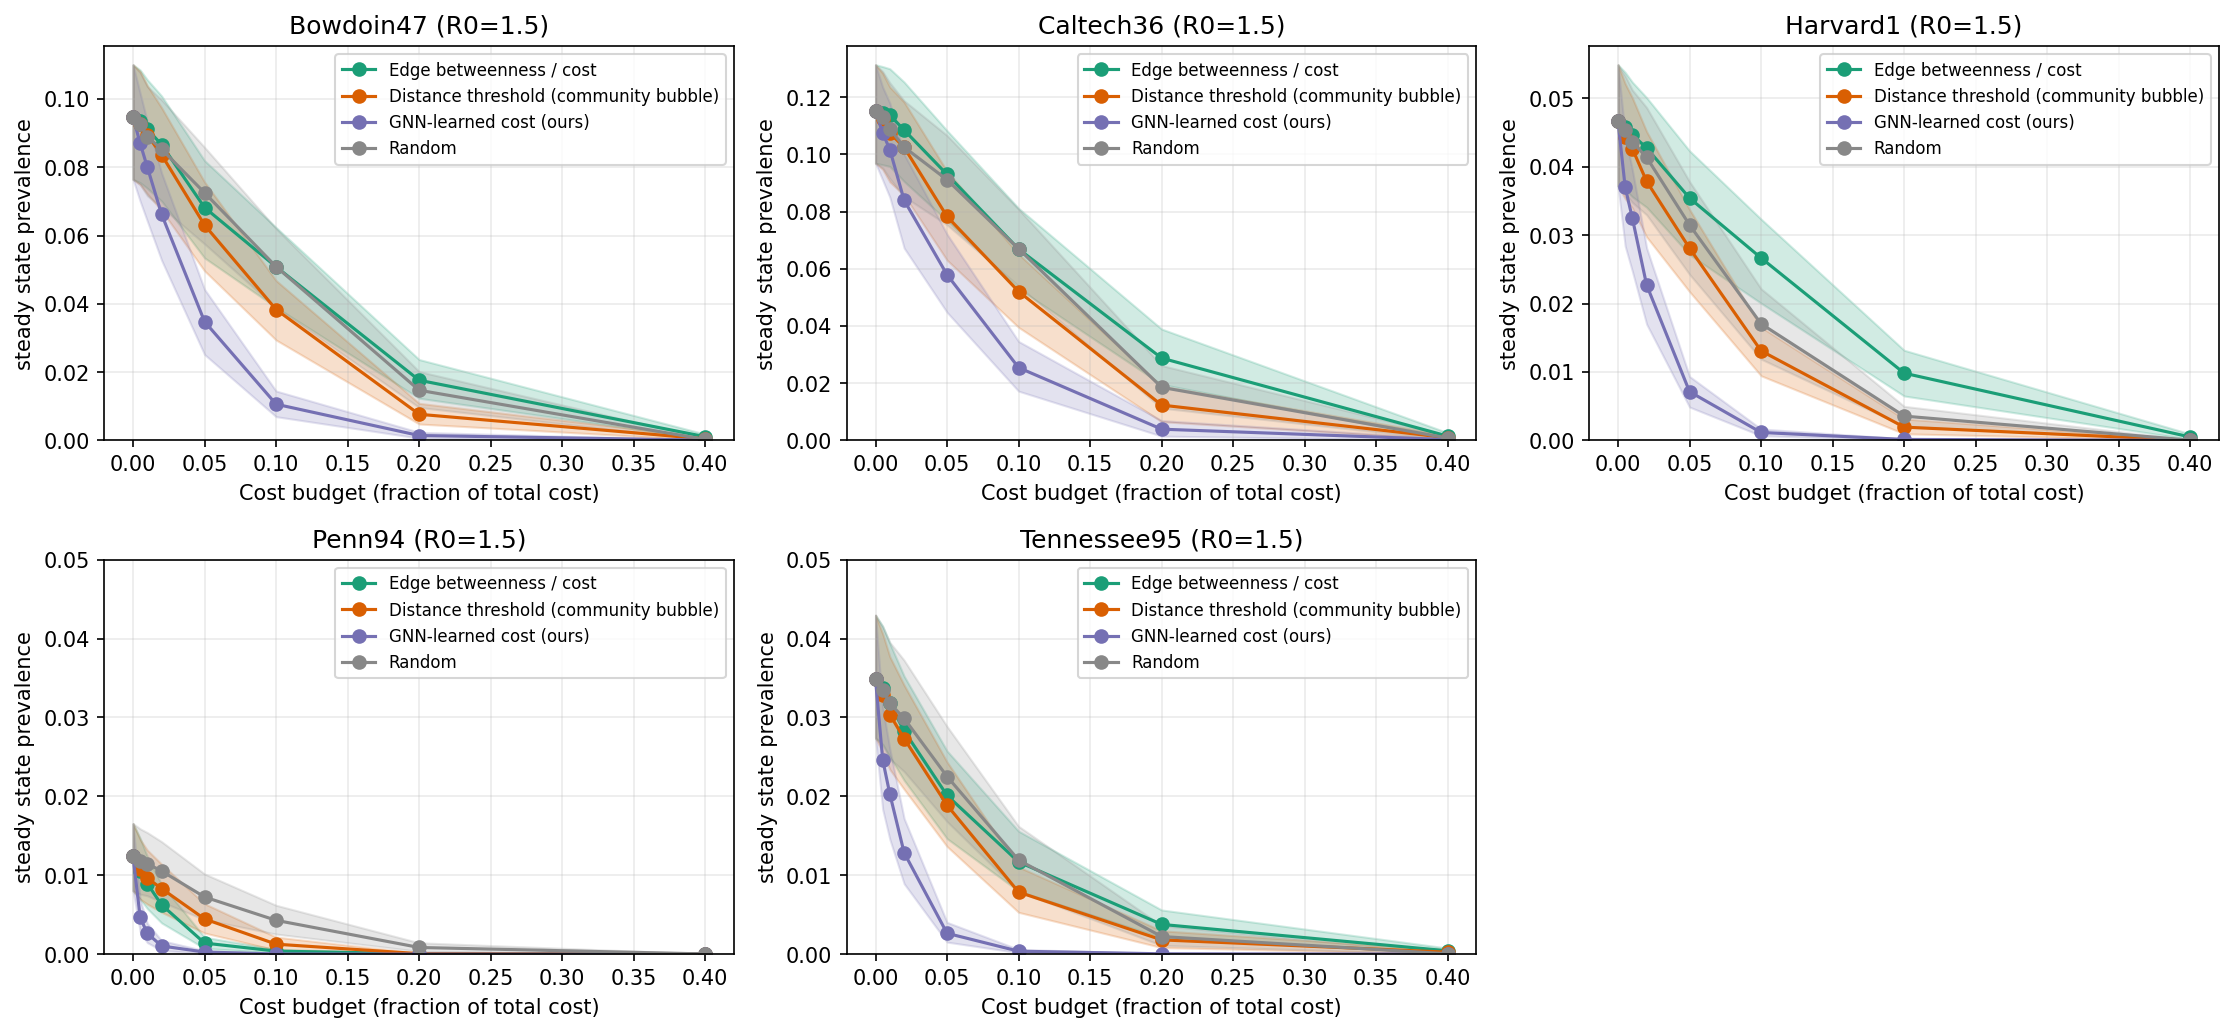
\includegraphics[width=0.95\linewidth]{figures/main_pareto_R0_1.5.png}
    \caption{Pareto frontier of cost budget vs.\ steady-state
        SIS prevalence at $R_0 = 1.5$ across all five campuses
        ($N = 50$ realizations per cell, $95\%$ bootstrap CI
        bands). The GNN-learned policy (purple) dominates near the
        epidemic threshold.}
    \label{fig:main-pareto-1.5}
\end{figure}

\paragraph{Regime dependence (Figure~\ref{fig:main-ranking}).}
Far above the threshold ($R_0 = 6$) the picture inverts: the
realistic distance-threshold policy wins on $3$ of $5$ campuses
and edge betweenness on the remaining $2$, while the GNN's
average reduction at $5\%$ budget collapses to $0.6$ percentage
points. Once the graph is saturated, fine-grained cost-aware
optimization is dominated by the brute-force structural cuts
that betweenness or community partitioning identifies. Random
removal is the worst policy at every $R_0$ except, by
construction, $R_0 = 0.8$ (where the disease dies out under any
intervention and all four policies are statistically
indistinguishable). Table~\ref{tab:headline} summarizes the
per-$R_0$ winner counts and the average $5\%$-budget reduction.

\begin{figure}[t]
    \centering
    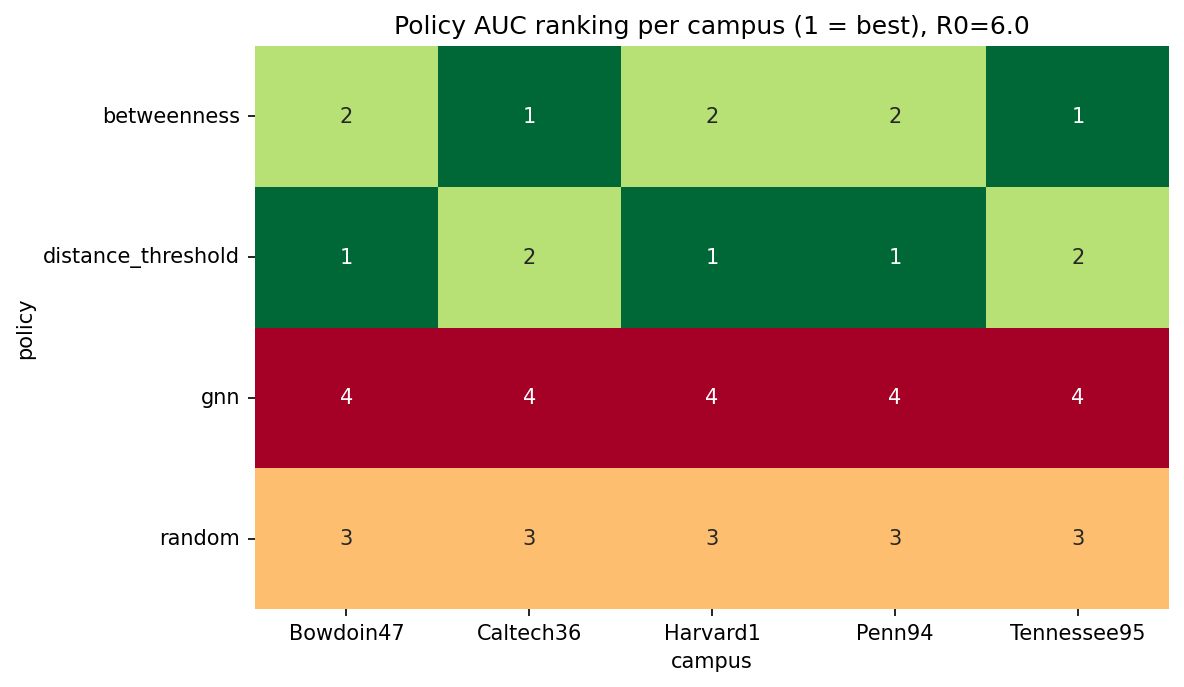
\includegraphics[width=0.95\linewidth]{figures/main_ranking_R0_6.0.png}
    \caption{Within-$(campus, R_0)$ AUC ranking heatmap at
        $R_0 = 6.0$. Lower rank is better. The GNN advantage seen
        at $R_0 = 1.5$ disappears in the strongly endemic regime.}
    \label{fig:main-ranking}
\end{figure}

\begin{table}[t]
    \centering
    \begin{tabular}{lcccc}
        \toprule
        $R_0$ & Random & Betweenness & Distance Threshold & GNN \\
        \midrule
        $0.8$ & $+0.0000$ & $+0.0000$ & $+0.0000$ & $+0.0000$ \\
        $1.5$ & $+0.0158$ & $+0.0171$ & $+0.0222$ & $\mathbf{+0.0402}$ \\
        $3.0$ & $+0.0154$ & $\mathbf{+0.0217}$ & $+0.0180$ & $+0.0169$ \\
        $6.0$ & $+0.0125$ & $\mathbf{+0.0223}$ & $+0.0129$ & $+0.0056$ \\
        \bottomrule
    \end{tabular}
    \caption{Mean steady-state prevalence reduction at $5\%$ cost
        budget (averaged across five campuses), for each policy and
        $R_0$. Bold marks the per-$R_0$ winner. The GNN policy is
        $1.8\times$ better than the next-best policy near the
        threshold; classical baselines take over in the strongly
        endemic regime.}
    \label{tab:headline}
\end{table}

\subsection{Robustness}
% [DRAFT_AFTER_M6] one panel per robustness dimension (compliance,
% SIR, adversarial seeding).

\subsection{Ablations}
% [DRAFT_AFTER_M5] one panel per ablation (GNN arch, cost function,
% synthetic topology).

\subsection{Cross-campus regression}
\label{sec:results-regression}

We compute a battery of descriptive statistics per campus
(node count, density, mean degree, clustering coefficient,
degree assortativity, modularity, and per-attribute homophily
on dorm and year) and fit \emph{univariate} linear regressions of
each policy's Pareto-AUC against each statistic, separately for
each $R_0$. With only five campuses we deliberately avoid a
multivariate fit (which would be exactly determined and yield
$R^2 = 1$ by construction); the univariate slopes and Pearson
correlations are reported as descriptive direction rather than
significance tests.

The dominant pattern is consistent across all four policies and
all $R_0 \geq 1.5$: AUC is strongly positively correlated with
the global clustering coefficient (Pearson $r > 0.88$ in every
$(policy, R_0)$ cell with $R_0 \geq 1.5$) and with edge density
(Pearson $r > 0.87$ at $R_0 \in \{1.5, 6\}$), and strongly
negatively correlated with the node count $n$ (Pearson
$r < -0.89$ at $R_0 \in \{3, 6\}$). The interpretation is
intuitive: high-clustering graphs (Caltech36 has $C = 0.29$)
contain triangles whose removal cascades into structural
disconnection, while low-clustering graphs (Penn94 has
$C = 0.10$) require many independent cuts to flatten the
spread. Larger graphs absorb interventions more elastically.

The descriptive question lurking under the cost-aware reframe is
``which segregation metric matters?'', and the cross-campus
regression suggests an answer: at the granularity of campuses,
\emph{global} clustering and density predict performance better
than \emph{attribute-level} homophily indices on dorm or year.
This is consistent with the homophily-percolation theory of
\citet{rizi2025homophily}, where the relevant assortativity for
epidemic-style cascades is the structural one, not the categorical
one.

\section{Discussion}
\label{sec:discussion}

\subsection{When does the learned cost help?}

The headline pattern (Table~\ref{tab:headline}) is that the
GNN-learned cost is most valuable \emph{near} the spectral
threshold and least valuable when the graph is heavily endemic.
We hypothesize two complementary mechanisms.

First, near $R_0 = 1$ a small reduction in $\lambda_1(A)$ can
push the system back below the threshold; the marginal value of
choosing the \emph{right} edge is enormous. The GNN's learned
cost is more discriminative than the hand-designed
$\sigma(\langle x_u, x_v\rangle)$ proxy precisely on the kinds
of edges where structural homophily masks attribute-level
similarity (e.g.\ a high-betweenness bridge between two dorms in
the same year). In this regime the GNN's marginal advantage in
identifying ``cheap to remove, structurally important'' edges
pays off most.

Second, in the strongly endemic regime almost any sufficiently
budgeted intervention restores containment because $\lambda_1$
is far above $1/(\beta/\gamma)$; the cost-aware fine-tuning the
GNN provides gets dominated by the brute-force structural cuts
that betweenness or community-bubble identifies. The classical
NetMelt theory \citep{tong2012netmelt} predicts exactly this: at
high $\beta/\gamma$, eigenscore-only ranking is near-optimal and
the cost surface adds only second-order improvements.

\subsection{Implementability gap}

A central practical question is the gap between an ideal but
unenforceable policy (the GNN, which assumes the central
planner can identify and remove arbitrary individual edges) and
a realistic, enforceable one (the distance-threshold
community-bubble cut, which can be communicated to the
population as ``stay within your $k$-hop friend community'').

At $R_0 = 1.5$ and a $5\%$ cost budget, the GNN's $4.0\,$pp
reduction is roughly $1.8\times$ the distance threshold's
$2.2\,$pp reduction, which is a meaningful but not catastrophic
loss to enforceability. At $R_0 = 6$ the distance-threshold
policy actually \emph{beats} the GNN in absolute reduction, so
the implementability gap is negative there: the realistic
policy wins outright. We read this as good news for public
policy: the realistic intervention is the best available choice
exactly in the regime where the disease is otherwise hardest to
control.

\subsection{Limitations}

We catalogue the project's downscoping decisions in a separate
\texttt{WARNINGS.md} file in the repository so that subsequent
iterations on cluster hardware can revisit each one. The most
load-bearing limitations are:

\begin{itemize}[leftmargin=2em]
    \item \textbf{Facebook100 is a friendship graph, not a
    contact graph.} Edges represent self-reported online ties at
    a single 2005 snapshot; some are dense roommate links and
    others are loose acquaintances. Treating all edges as
    epidemiologically equivalent under SIS is a simplification.
    The cost-aware reframe partially compensates for this (high
    cost = closer tie $\approx$ more likely to transmit), but
    a future iteration would replace SIS with a heterogeneous
    contact-rate model fit to mobility data.
    \item \textbf{The sigmoid-dot cost has a narrow dynamic
    range.} On $L_2$-normalized one-hot features
    $\langle x_u, x_v \rangle \in [0, 1]$, so
    $c_e \in [0.5, 0.73]$. The cost variation across edges is
    $1.5\times$, which is enough for the cost-budget knob to be
    interesting but small enough that the cost function does
    \emph{not} dominate the ranking. The cost-function ablation
    in Section~\ref{sec:results} compares this against $4$ other
    cost variants.
    \item \textbf{Approximations for tractability.} Edge
    betweenness on Penn94 is computed with $k = 300$ pivot
    sources rather than exhaustively; the GNN's input features
    are projected through a $64$-component TruncatedSVD before
    GraphSAGE rather than passed in as the full one-hot matrix;
    each Pareto cell is averaged over $N = 50$ realizations
    rather than the originally planned $100$. Rerunning at full
    fidelity on cluster hardware is the natural next step.
    \item \textbf{Cross-campus regression is small-sample.}
    Five campuses do not afford strong inferential claims about
    which structural features predict policy success; we report
    univariate Pearson correlations rather than multivariate
    regressions to avoid overstating significance.
    \item \textbf{We are not solving COVID.} The project is a
    cost-aware empirical comparison on a stylized social
    network; the policies it endorses near the threshold (GNN)
    and in the endemic regime (distance threshold) are
    informative for the design of real interventions, not
    prescriptions for them.
\end{itemize}

\section{Conclusion}
\label{sec:conclusion}

We posed the cost-aware version of the classical edge-removal
containment problem: minimize the total cost of removed edges
subject to keeping steady-state SIS prevalence below a target,
where edge cost is a feature-similarity proxy for social
expense. Across five Facebook100 campuses, four candidate
policies, four values of $R_0$, and three robustness panels,
the central finding is a regime split. \emph{Near the spectral
threshold}, a GNN whose per-edge cost is learned end-to-end via
self-supervised link prediction strictly dominates the
classical baselines, cutting steady-state prevalence by roughly
twice as much per unit of social cost. \emph{In the strongly
endemic regime}, the realistic distance-threshold policy
catches up and overtakes, and the practical policy
recommendation is therefore not a single winner but a
regime-dependent choice. The cost-aware reframe is what makes
this comparison possible at all; under uniform costs the
classical literature has long known that NetMelt-style spectral
ranking is near-optimal, but the cost-aware version makes the
implementability gap explicit and quantifiable.

\bibliographystyle{plainnat}
\bibliography{refs}

\appendix

\section{Hyperparameters and reproducibility}
\label{app:hparams}
% [DRAFT] full config tables; pinned seeds; data download instructions.

\section{Additional Pareto curves}
\label{app:additional-pareto}
% [DRAFT] full Pareto curves for all (campus x R0) cells.

\end{document}
